\documentclass[hyperref={xetex,colorlinks,linkcolor=blue},green,compress]{beamer}
\usepackage{latexsym,pifont,units,amsmath,amsfonts,amssymb}
\usepackage{xltxtra} %fontspec,xunicode are loaded here.
%\usepackage{graphicx} % beamer loads graphicx already.
\graphicspath{{./figs/}{../figs/}{./}{../}} %note that the trailing “/” is required
%\usepackage{pdfsync,comment}
\usepackage{tikz}
\usetikzlibrary{arrows,decorations.pathmorphing,backgrounds,positioning,fit}
\usepackage{listings}
\lstset{language=c, basicstyle=\small, stringstyle=\ttfamily,emphstyle=\color{red},numberstyle=\tiny,numbersep=.5em}
\usepackage{xeCJK}
\setsansfont{DejaVu Sans}
%\setromanfont{DejaVu Serif}
%\setmainfont{DejaVu Serif}
%\setmonofont{DejaVu Sans Mono}
\setCJKmainfont[BoldFont={WenQuanYi Zen Hei}, ItalicFont={WenQuanYi Zen Hei}]{SimSun}
\setCJKfamilyfont{hei}{WenQuanYi Zen Hei}
\setCJKfamilyfont{song}{SimSun}

%\newcommand{\ziju}[1]{\renewcommand{\CJKglue}{\hskip #1}}
\usetheme{default}
\usecolortheme{rose}
\usefonttheme[onlysmall]{structurebold}
\usenavigationsymbolstemplate{}
\setbeamertemplate{footline}[frame number]
\setbeamertemplate{navigation symbols}{}
\setbeamertemplate{blocks}[rounded][shadow=true]
%\setbeameroption{show notes}
%\beamertemplateballitem

\begin{document}

\title{C Programming}\subtitle{File Handling}
\author{王晓林}

\lstset{language=C, numbers=left}

\begin{frame}
\titlepage

\vfill

\tiny{
\ding{41} wx672ster@gmail.com\\
\ding{37} 13577067397\\
}
\end{frame}

\begin{frame}\frametitle{References}
  \begin{thebibliography}{}
  \bibitem[cPrimerPlus]{cPrimerPlus}
    \href{http://218.194.106.3/pub/Books/tech/c/cPrimerPlus/}{C Primer
      Plus 5th Edition, November 23, 2004, Sams}
  % \bibitem[moodle]{moodle}
  %   \href{http://cs2.swfu.edu.cn/moodle/course/view.php?id=25}{计科系网上教学}
  \end{thebibliography}
\end{frame}

\begin{frame}\frametitle{What Is a File?}
  \begin{itemize}
  \item In UNIX, everything is a file.
  \item In UNIX, everything is a stream of bytes.
  \end{itemize}
  \begin{exampleblock}{Stream}
    \begin{itemize}
    \item is a continuous sequence of bytes.
    \item is a portable way of reading and writing data.
%    \item is a file or a physical device (e.g. printer or monitor) which is manipulated with a \emph{pointer} to the stream
    \item is a common, logical interface to a \emph{file} (disk file,
      directory, the screen, the keyboard, a sound card, a NIC, etc.)
    \end{itemize}
  \end{exampleblock}
\end{frame}

\begin{frame}\frametitle{Text View, Binary View}
  \begin{itemize}
  \item text output: printable characters + CR/LF/Tab
  \item binary output: not human readable
  \end{itemize}
  \begin{exampleblock}{Text vs. Binary}
    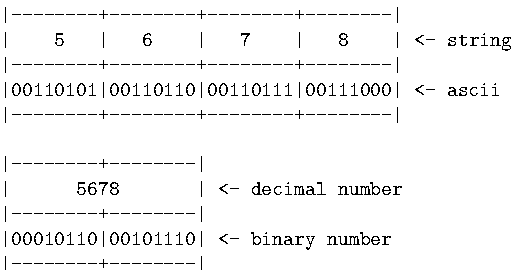
\includegraphics[width=\textwidth]{5678}
  \end{exampleblock}
\end{frame}

\begin{frame}\frametitle{Functions}
  As a programmer, you will have to write programs that
  \begin{itemize}
  \item create files
  \item write into files
  \item read from files
  \end{itemize}
  \begin{exampleblock}{Functions to use:}
    \begin{center}
      \begin{tabular}{llll}
        fopen()&getc()&putc()&fclose()\\
        fprintf()&fscanf()&fgets()&fputs()\\
        rewind()&fseek()&ftell()&fflush()\\
        fgetpos()&fsetpos()&feof()&ferror()\\
        ungetc()&setvbuf()&fread()&fwrite()
      \end{tabular}
    \end{center}
  \end{exampleblock}
\end{frame}

\begin{frame}\frametitle{FILE --- An Internal C Data Structure}
  \begin{itemize}
  \item We just need to declare a variable or pointer of \emph{FILE} type in our programs.
  \item We do not need to know any more specifics about \emph{FILE} definition.
  \item We must open a \emph{stream} before doing any I/O,
  \item then access it
  \item and then close it.
  \end{itemize}
\end{frame}

\begin{frame}
  \begin{example}
    \includegraphics[height=.9\textheight]{count_c}
  \end{example}
\end{frame}

\begin{frame}\frametitle{In the program ...}
  \begin{enumerate}
  \item checks the value of \alert{$argc$}
  \item Using \alert{$argv[0]$} instead of the program name
    explicitly
  \item \alert{$exit()$}
  \item \alert{$fopen()$} and \alert{$fclose()$}
  \item \alert{$getc()$} and \alert{$putc()$}
  \item \alert{$EOF$}
  \item \alert{$stdin$}, \alert{$stdout$}, and \alert{$stderr$}
  \end{enumerate}
\end{frame}

\begin{frame}\frametitle{stdin, stdout, stderr}
  \begin{exampleblock}{Deferent names}
    \begin{itemize}
    \item Standard files
    \item Standard file pointers
    \item Predefined file descriptors
    \item Predefined streams
    \end{itemize}
  \end{exampleblock}
  \begin{itemize}
  \item \begin{tabular}{l}
      stdin\\
      stdout\\
      stderr
    \end{tabular}
    are automatically open to all C programs.
  \item There is no need to use fopen on them.
  \end{itemize}
\end{frame}

\begin{frame}[fragile]\frametitle{fopen()}
  \begin{itemize}
  \item returns a file pointer
  \item returns NULL if failed to open a file
  \end{itemize}
  \begin{small}
    \begin{exampleblock}{}
      \begin{lstlisting}
/* declare a stream and prototype fopen */
FILE *stream, *fopen();
      
stream = fopen("myfile.dat","r");
      \end{lstlisting}
    \end{exampleblock}
    \begin{exampleblock}{}
      \begin{lstlisting}
/* it is good practice
   to to check file is opened correctly */
if ((stream = fopen("myfile.dat", "r"))
            == NULL)
{            
  printf("Can't open %s", "myfile.dat");
  exit(1);
}
      \end{lstlisting}
    \end{exampleblock}
  \end{small}
\end{frame}

\begin{frame}\frametitle{Mode Strings for fopen()}
  \begin{description}
  \item["r"] Open a text file for reading
  \item["w"] Open a text file for writing
  \item["a"] appending to the end of a file
  \item["r+"] Open a text file for update
  \item["w+"] Open a text file for update
  \item["a+"] Open a text file for update
  \item["rb", "rb+", "r+b"] binary read
  \item["wb", "wb+", "w+b"] binary write
  \item["ab", "ab+", "a+b"] binary append
  \end{description}
\end{frame}

\begin{frame}[fragile]
  \frametitle{getc() and putc()}
  \begin{exampleblock}{}
    \begin{lstlisting}
ch = getc(fp);    // read from fp
ch = getc(stdin); // read from keyboard
ch = getchar();   // read from keyboard
putc(ch,fpout);   // write to fpout
putc(ch,stdout);  // write to screen
putchar(ch);      // write to screen
    \end{lstlisting}
  \end{exampleblock}
\end{frame}

\begin{frame}[fragile]
  \frametitle{EOF}
  \begin{exampleblock}{Good design to avoid problems attempting to read an empty
      file}
    \begin{lstlisting}
int ch;
FILE *fp;

fp = fopen("wacky.txt", "r");

while (( ch = getc(fp)) != EOF)
{
  putchar(ch);  // process input
}
\end{lstlisting}
  \end{exampleblock}
\end{frame}

\begin{frame}[fragile]
  \frametitle{EOF}
  \begin{exampleblock}{Bad design}
    \begin{lstlisting}
int ch;
FILE *fp;

fp = fopen("wacky.txt", "r");

while (ch != EOF)  // ch undetermined 
{
  ch = getc(fp);   // get input
  putchar(ch);     // process input
}
 \end{lstlisting}
  \end{exampleblock}
  Two problems:
  \begin{enumerate}
  \item the first time ch is compared with EOF, it has not yet been
    assigned a value.
  \item if getc() does return EOF, the loop tries to process EOF as if
    it were a valid character.
  \end{enumerate}
\end{frame}

\begin{frame}[fragile]
  \frametitle{fclose()}
  \begin{exampleblock}{}
    \begin{lstlisting}
if (fclose(fp) != 0)
  printf("Error in closing file %s\n", argv[1]);
    \end{lstlisting}
  \end{exampleblock}
\end{frame}

\begin{frame}
  \begin{exampleblock}{Open two files simultaneously}
    \includegraphics[height=.9\textheight]{reducto_c}
  \end{exampleblock}
\end{frame}

\begin{frame}\frametitle{fprintf(), fscanf()}
  \begin{itemize}
  \item fprintf(fp, "Syntax error on line \%d", lineno);
  \item fprintf(stderr, "Syntax error on line \%d", lineno);
  \item printf("Syntax error on line \%d", lineno);
  \item fscanf(fp, "\%s", string);
  \item fscanf(stdin, "\%s", string);
  \item scanf("\%s", string);
  \end{itemize}
\end{frame}

\begin{frame}
  \begin{exampleblock}{uses fprintf(), fscanf(), and rewind()}
    \includegraphics[height=.9\textheight]{addaword_c}    
  \end{exampleblock}
\end{frame}

\begin{frame}\frametitle{fgets(), fputs()}
  \begin{exampleblock}{}
    \begin{itemize}
    \item fgets(buf, MAX, fp);
      \begin{itemize}
      \item \alert{buf} is the name of a char array
      \item \alert{MAX} is the maximum size of the string
      \item \alert{fp} is the pointer-to-FILE
      \end{itemize}
      fgets() returns the value NULL when it encounters EOF
    \item fgets(buf, MAX, stdin);
    \item gets(buf);
    \end{itemize}
  \end{exampleblock}
  \begin{exampleblock}{}
    \begin{itemize}      
    \item fputs(buf, fp);
      \begin{itemize}
      \item \alert{buf} is the string address
      \item \alert{fp} identifies the target file
      \end{itemize}
    \item fputs(buf, stdout);
    \item puts(buf);
    \end{itemize}
  \end{exampleblock}
\end{frame}

\begin{frame}[fragile]
  \begin{exampleblock}{using fgets() and fputs()}
    \begin{lstlisting}
#include <stdio.h>
#define MAXLINE 20
int main(void)
{
  char line[MAXLINE];

  while (fgets(line, MAXLINE, stdin) != NULL &&
           line[0] != '\n')
         fputs(line, stdout);
  return 0;
}
    \end{lstlisting}
  \end{exampleblock}
\end{frame}

\begin{frame}[fragile]
  \frametitle{Jump To a Certain Position In a
    File}\framesubtitle{fseek(), ftell()}
  \begin{exampleblock}{}
    \begin{lstlisting}
long int pos;
pos = ftell(fp); // record current position
// after some operation, you can ...
fseek(fp, pos, SEEK_SET); // go back to pos
    \end{lstlisting}
  \end{exampleblock}
  \begin{description}
  \item[fp:] file pointer
  \item[pos:] offset, \alert{long} int
  \item[SEEK\_...:] identifies the starting point.
    \begin{description}
    \item[SEEK\_SET:] Beginning of file
    \item[SEEK\_CUR:] Current position
    \item[SEEK\_END:] End of file
    \end{description}
  \end{description}
\end{frame}

\begin{frame}[fragile]
 \begin{example}
    \begin{lstlisting}
// go to the beginning of the file
fseek(fp, 0L, SEEK_SET);   
// go 10 bytes into the file
fseek(fp, 10L, SEEK_SET);  
// advance 2 bytes from the current position
fseek(fp, 2L, SEEK_CUR);   
// go to the end of the file
fseek(fp, 0L, SEEK_END);   
// back up 10 bytes from the end of the file
fseek(fp, -10L, SEEK_END); 
    \end{lstlisting}
  \end{example}
  \begin{description}
  \item[L:] long integer
    \begin{description}
    \item[positive:] move forward
    \item[negative:] move backword
    \item[zero:] stay put
    \end{description}
  \end{description}
\end{frame}

\begin{frame}
  \begin{exampleblock}{reverse.c -- displays a file in reverse order}
    \includegraphics[height=.9\textheight]{reverse_c}        
  \end{exampleblock}
\end{frame}

\begin{frame}\frametitle{fread(), fwrite()}
  \begin{exampleblock}{fprintf() vs. fwrite()}
    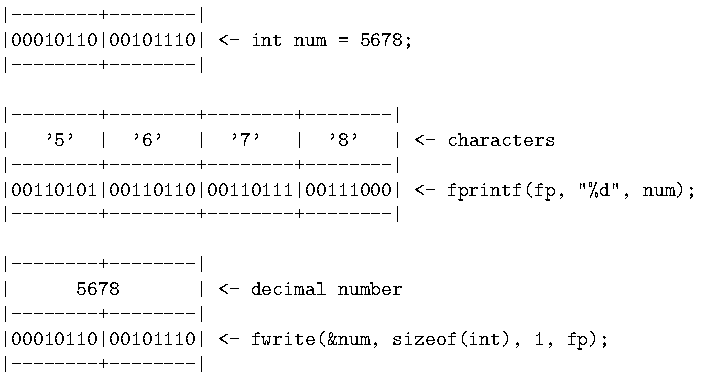
\includegraphics[width=\textwidth]{12345}            
  \end{exampleblock}
\end{frame}
\end{document}
